\chapter{Classification}

\section{Problem}
We choose to solve the obvious classification problem for the MNIST data set, which is to classify the digit of each observation. 

\section{Classification techniques}
% Apply at least three of the following methods:
% (Use cross-validation to select relevant parameters in an inner cross-validation
% loop and give in a table the performance results for the methods evaluated
% on the same cross-validation splits on the outer cross-validation loop, i.e. you
% should use two levels of cross-validation).
There have been looked into a few different methods for classification and by means of paired t-tests it have been found if one method is significant different from the others.

\subsection{Decision Trees}
Since we have a lot of attributes, which do not hold any significant meaning besides an seemingly arbitrary integer value, the decision tree solution is likely to not be very precise in determining the class. It will also be quite a bit tree since it has to value in each  of the different attributes, and determine what the meaning of that specific attribute might be in the classification.
\begin{figure}[H]
\centering
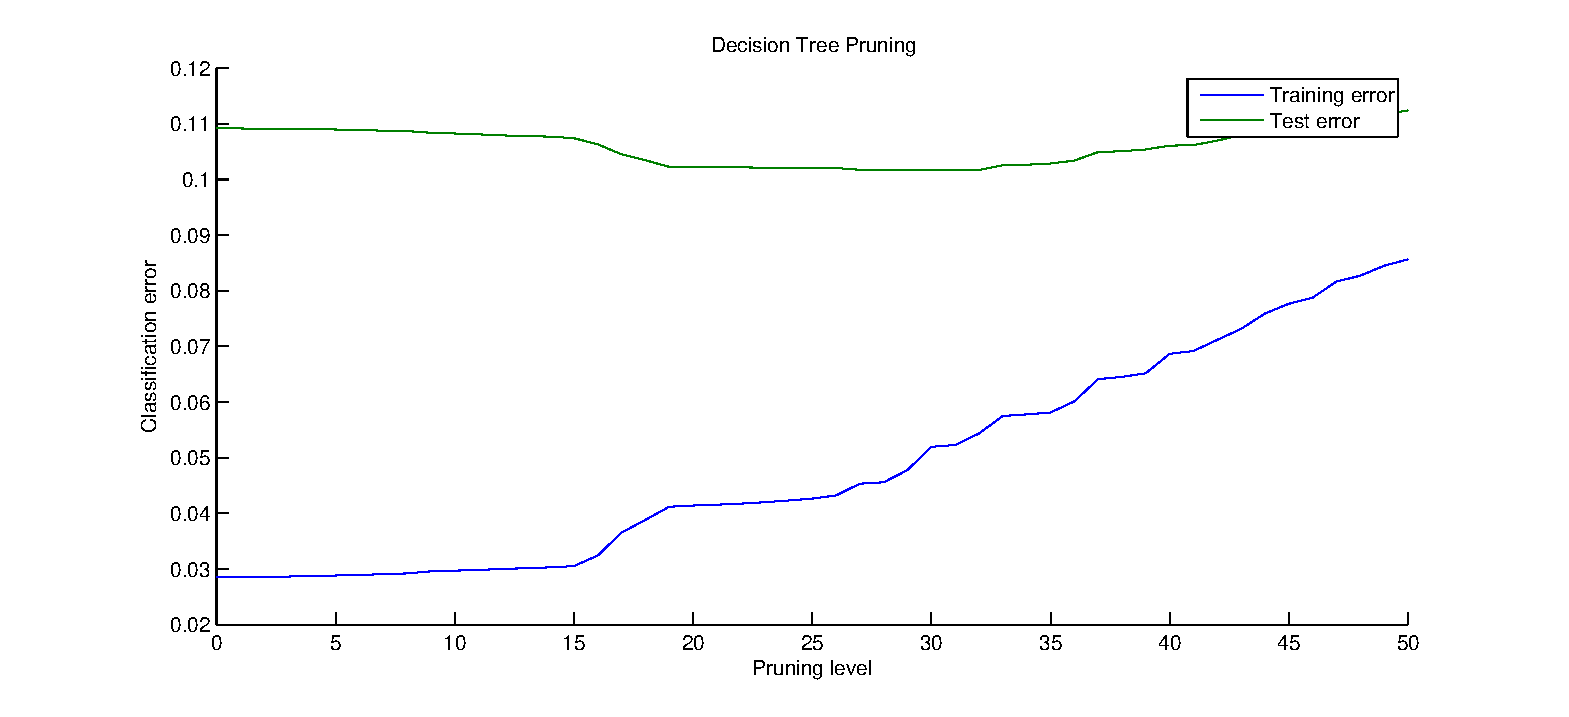
\includegraphics[width=\linewidth]{code/decision_tree_pruning}
\caption{test\label{fig:linf}}
\end{figure}

\subsection{K-Nearest Neighbors (KNN)}
As the computation demand of KNN is significant larger then the other two, we first estimated parameters for a subset of the data and then did the same again for a smaller subset of the parameters. This way we was able to find the optimal parameter in feasible time.

\begin{figure}[H]
\centering
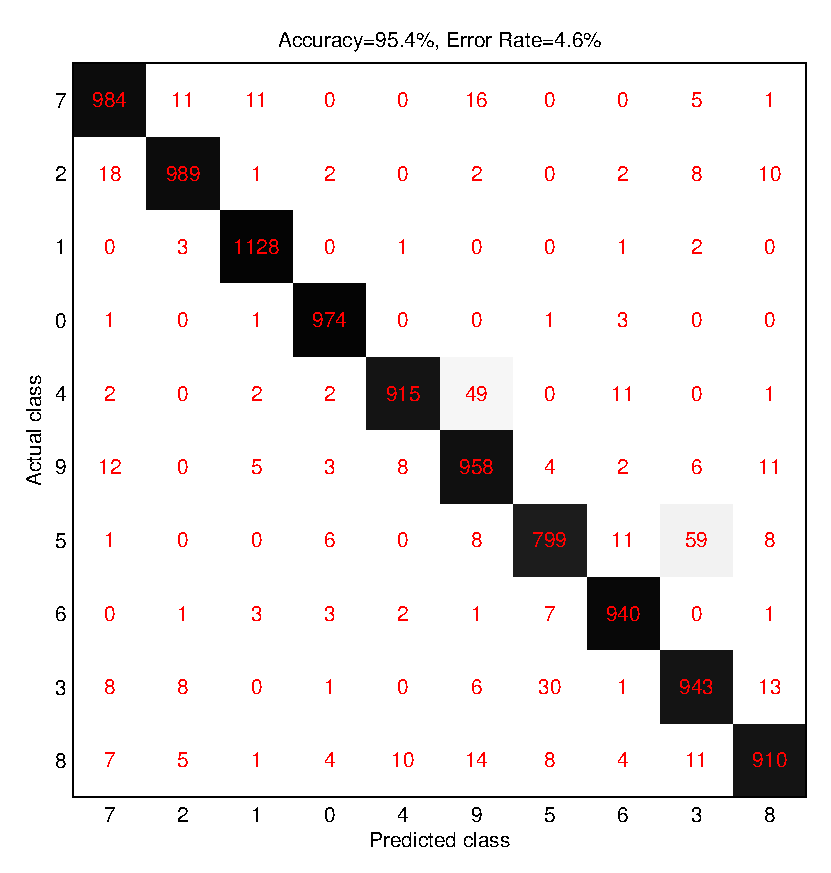
\includegraphics[width=\linewidth]{code/confusm_k5}
\caption{The confusion matrix for KNN classifications with 5 neighbors. It can be seen how 3 and 5 get confused the most.\label{fig:knn}}
\end{figure}
\begin{figure}[H]
\centering
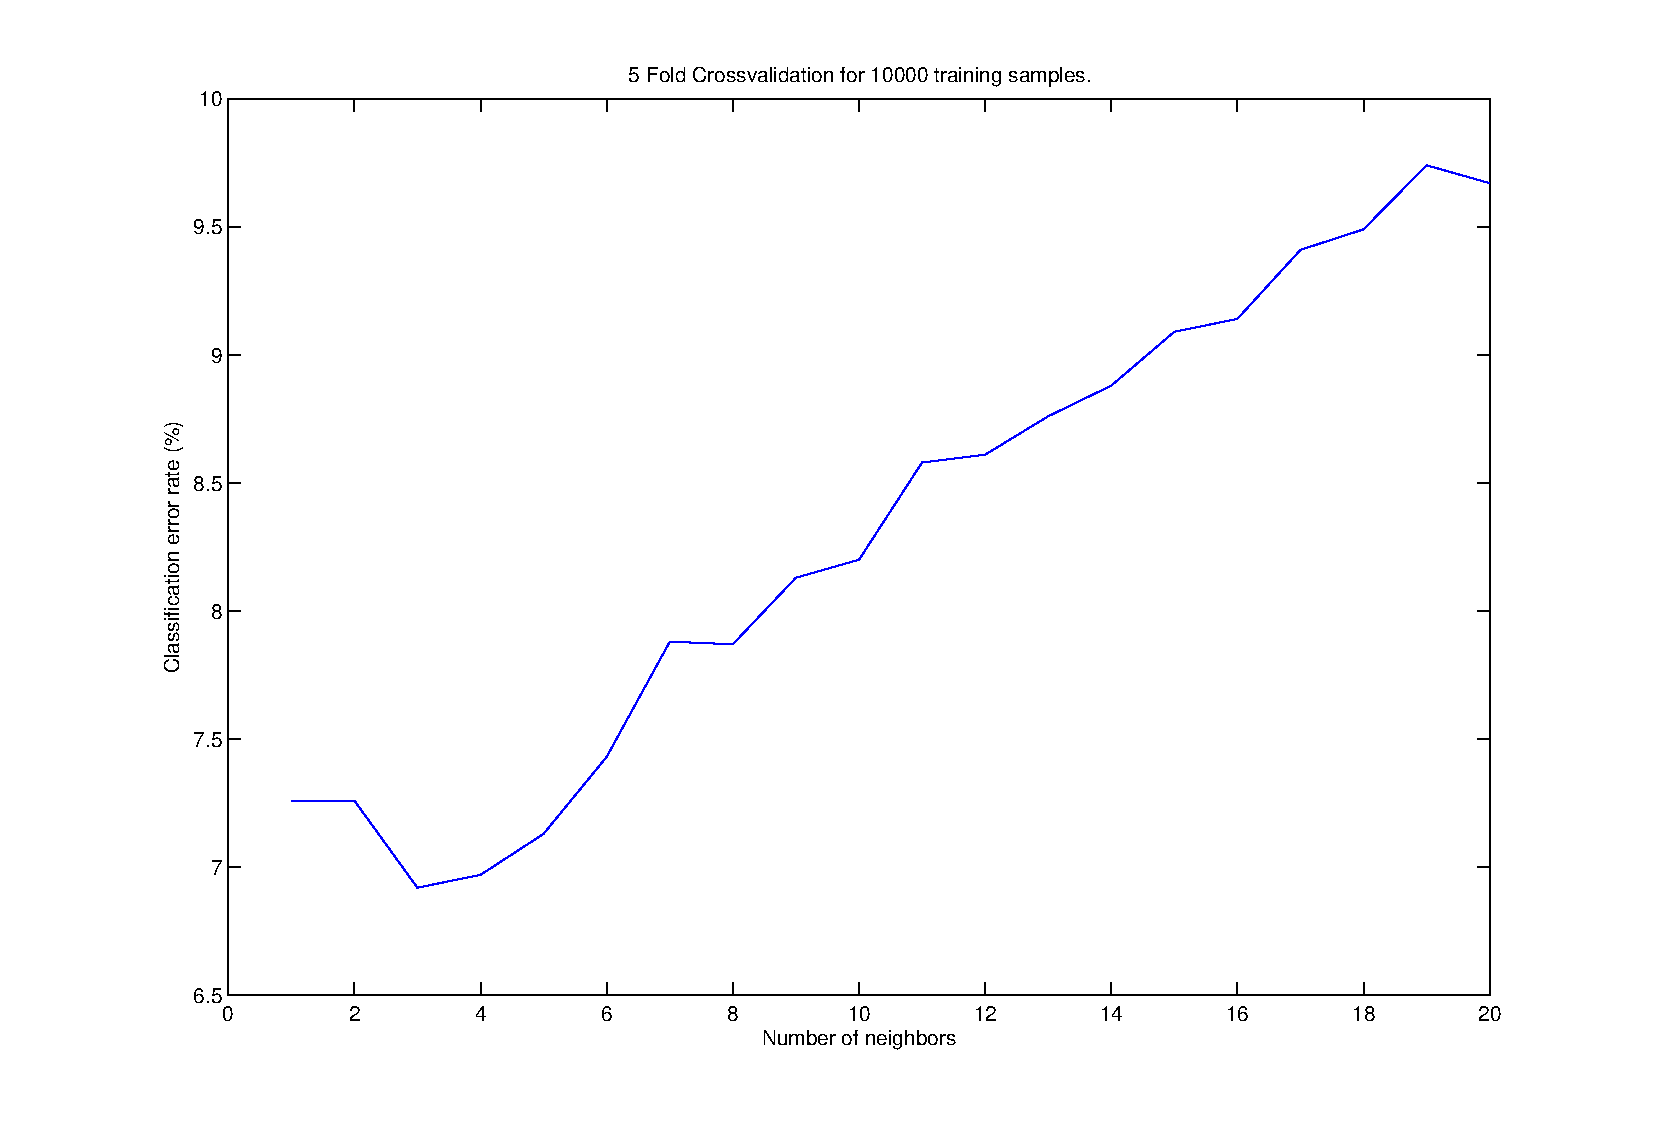
\includegraphics[width=\linewidth]{code/5fold_knn_10000samples}
\caption{The five fold cross validation for 10000 samples.\label{fig:knn_small}}
\end{figure}
\begin{figure}[H]
\centering
\includegraphics[width=\linewidth]{code/5fold_knn_60000samples}
\caption{The cross validation for the full dataset.\label{fig:knn_large}}
\end{figure}



\subsection{Naïve Bayes}

%\subsection{Artificial Neural Networks (ANN)}


\section{New data observation}
% For the models you are able to interpret explain how a new data observation
% is classified.
% (If you have multiple models fitted, (i.e., one for each cross-validation split)
% either focus on one of these fitted models or consider fitting one model for
% the optimal setting of the parameters estimated by cross-validation to all the
% data.)
For some models it is more trivial to explain what is going on behind the scene, but with this dataset of 272 features some of the simplicity fades away. Using decision trees it is trivial to by hand to take a new sample and move your way down the tree until a leaf is reached. At each split one could look at the distributions of samples in the two subtrees and tell what the meaning of the feature is. We argue that because of our data size it is not feasible to manually move one observation down the tree even though it being trivial. 

For neural networks we could also manually compute the activation of each neuron and so forth. This could be done efficiently with matrix multiplication but because of the data size it would take forever. 

While understanding the theory and how a model classify a observation, it makes less sense in our case and we have put our faith into the toolbox. 

\section{Performance comparison}
% Statistically compare the performance of the two best performing models (i.e.,
% use a paired t-test). Compare in addition if the performance of your models
% are better than simply predicting all outputs to be the largest class in the
% training data.
In Table~\ref{tab:ttest} the paired t-test values can be seen. As none of them span across zero they are all significant different.
\begin{table}[h]
\centering
\begin{tabular}{|l|c|}
\hline
KNN vs Trees & [-0.0604   -0.0540] \\ \hline
KNN vs NB	 & [-0.1217   -0.1173]\\ \hline   %KNN vs
NB vs Trees  & [-0.0657   -0.0589] \\ \hline					%Naive vs
\end{tabular}\\
\caption{Paired T-Test\label{tab:ttest}}
\end{table}